\chapter{Study Management}

 In this module the \entitylink{Study} aggregate is used to configure a
 study. It defines the valid types of specimens that can be collected, when
 they are to be collected from participants, and how the collected specimens
 are processed.

 This section first describes the study aggregate and then defines the commands
 it handles.

\section{Study Aggregate}

\begin{figure}[h]
  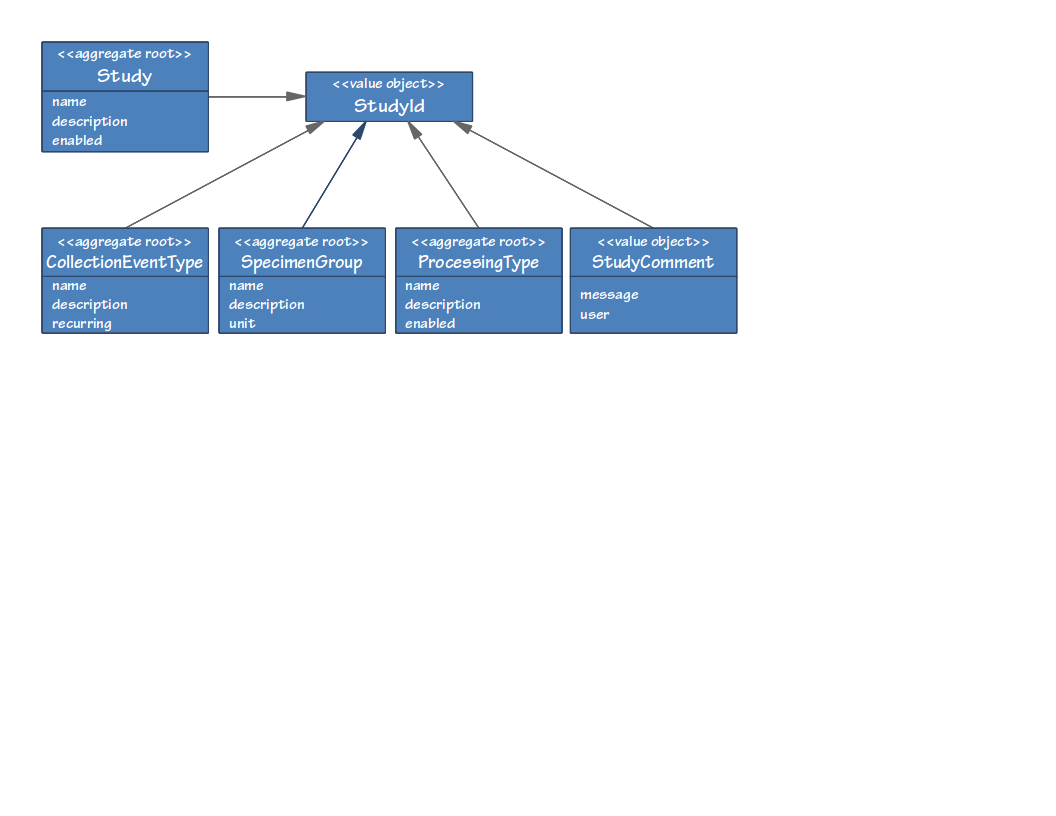
\includegraphics[trim={9mm 104mm 80mm 9mm}, clip,
    width=1\textwidth]{images/study-aggregate}
  \caption{Study aggregate}
  \label{fig:study-aggregate}
\end{figure}

\begin{description}[listparindent=\parindent]

  \item[\entitytarget{Study}] \hfill \\ Represents a collection of participants
    and specimens collected for a particular research study. The study name is
    a short descriptive name that is used to display summary information. The
    description contains text used to give more details on the name. Usually
    the name is an acronym and the description contains the words used in the
    acronym.

    A study can be enabled or disabled. When disabled, changes to its
    configuration are possible but patients and specimens cannot be added. When
    enabled, no further configuration changes are allowed, and participants and
    specimens can be added.

    A study may have one or more comments assigned to it during it's lifetime.

    Note: this aggregate has other associations that are introduced in later
    sections.

  \item[\entitytarget{SpecimenGroup}] \hfill \\ Ownership, summary, storage,
    and classification information that applies to an entire group or
    collection of \entitylink{Specimen}s.

    This entity is used to record the specimen types used by the study. It can
    specify the specimens collected from participants, and the specimens that
    are processed from them.

    The anatomical source, preservation medium and specimen type are defined
    using other value objects discussed in Section \ref{sec:specimen-group}.

  \item[\entitytarget{CollectionEventType}] \hfill \\ A classification name,
    unique to the \entitylink{Study}, for a visit by study participants. For
    specimen collection to be allowed on a study, at least one collection event
    type must be defined. Each collection event type has one or more specimen
    groups (see Section \ref{sec:collection-event-type}).

  \item[\entitytarget{ProcessingType}] \hfill \\ Describes a regularly
    performed specimen processing procedure with a unique name (unique to the
    \entitylink{Study}). There should be one or more associated
    \entitylink{SpecimenLinkType}s that (1) further define legal procedures and
    (2) allow recording of procedures performed on different types of
    \entitylink{Specimen}s.

  \item[\valobjtarget{StudyComment}] \hfill \\ The comment contains a message
    and the user that added the comment. The date and time the comment was made
    is recorded as meta data.

\end{description}

\subsection{SpecimenGroup}
\label{sec:specimen-group}

The SpecimenGroup entity is composed of other value objects as shown in Figure
\ref{fig:specimen-group}. \entitylink{SpecimenGroup} entities are accessed
via the \entitylink{Study} aggregate.

\begin{figure}[h]
  \centering
  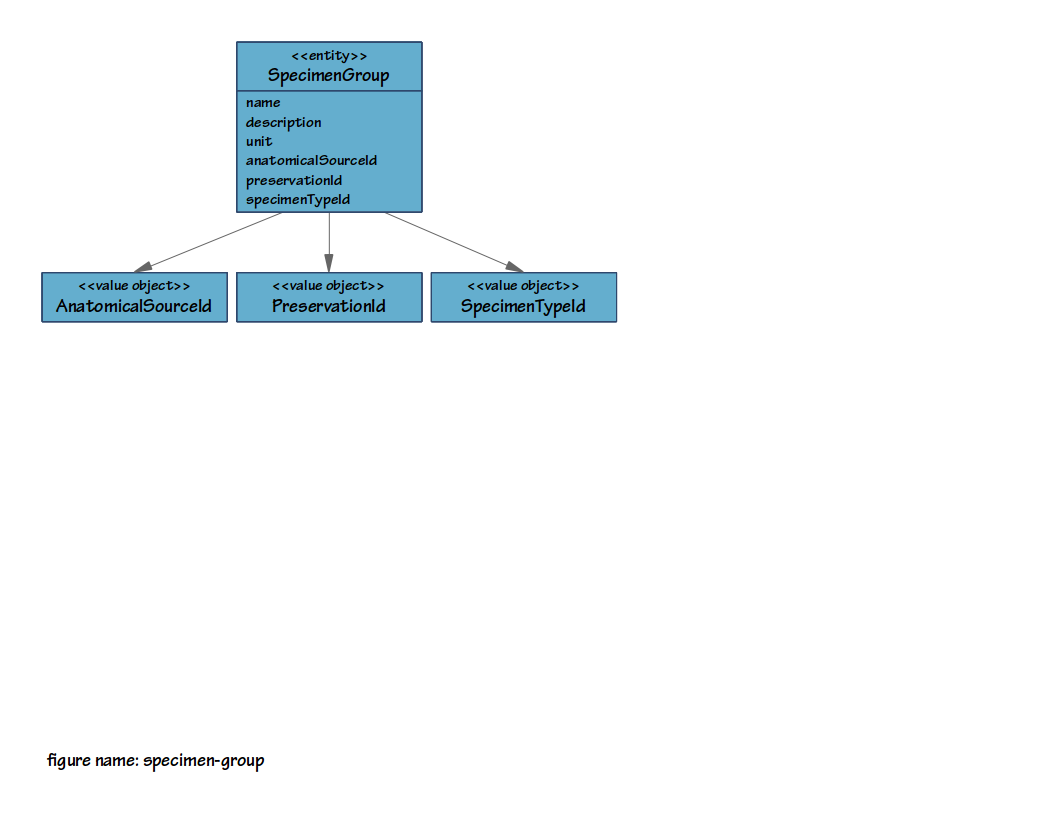
\includegraphics[trim={9mm 162mm 80mm 9mm}, clip,
    width=1\textwidth]{images/specimen-group}
  \caption{SpecimenGroup entity}
  \label{fig:specimen-group}
\end{figure}

\begin{description}

  \item[\valobjtarget{AnatomicalSourceId}] \hfill \\ The ID belonging to a
    \valobjlink{AnatomicalSource} which is a standardized set of regions from a
    \entitylink{Participant} \emph{where} a \entitylink{Specimen} is collected
    from. Potential examples include: colon, ear, leg, kidney, etc.

  \item[\valobjtarget{PreservationId}] \hfill \\ The ID belonging to a
    \valobjlink{Preservation} value object which describes how a
    \entitylink{Specimen} should be preserved/stored by describing temperature
    requirements ($^\circ$C), as well as a preservation method (see
    \valobjlink{PreservationType}).

  \item[\valobjtarget{SpecimenTypeId}] \hfill \\ The ID belonging to a
    \valobjlink{SpecimenType} which is standardized set of classifications that
    describe \emph{what} a \entitylink{Specimen} is. Potential examples
    include: urine, whole blood, plasma, nail, protein, etc.

\end{description}

\subsection{CollectionEventType Details}
\label{sec:collection-event-type}

The \texttt{\textbf{\valobjtarget{SpecimenGroupCollectionEventType}}} value
object is used to define which types of specimens (i.e. which
\valobjlink{SpecimenGroup}s) need to be collected as part of a
\entitylink{CollectionEventType}. See Figure \ref{fig:collection-event-type}.

\begin{figure}[h]
  \centering
  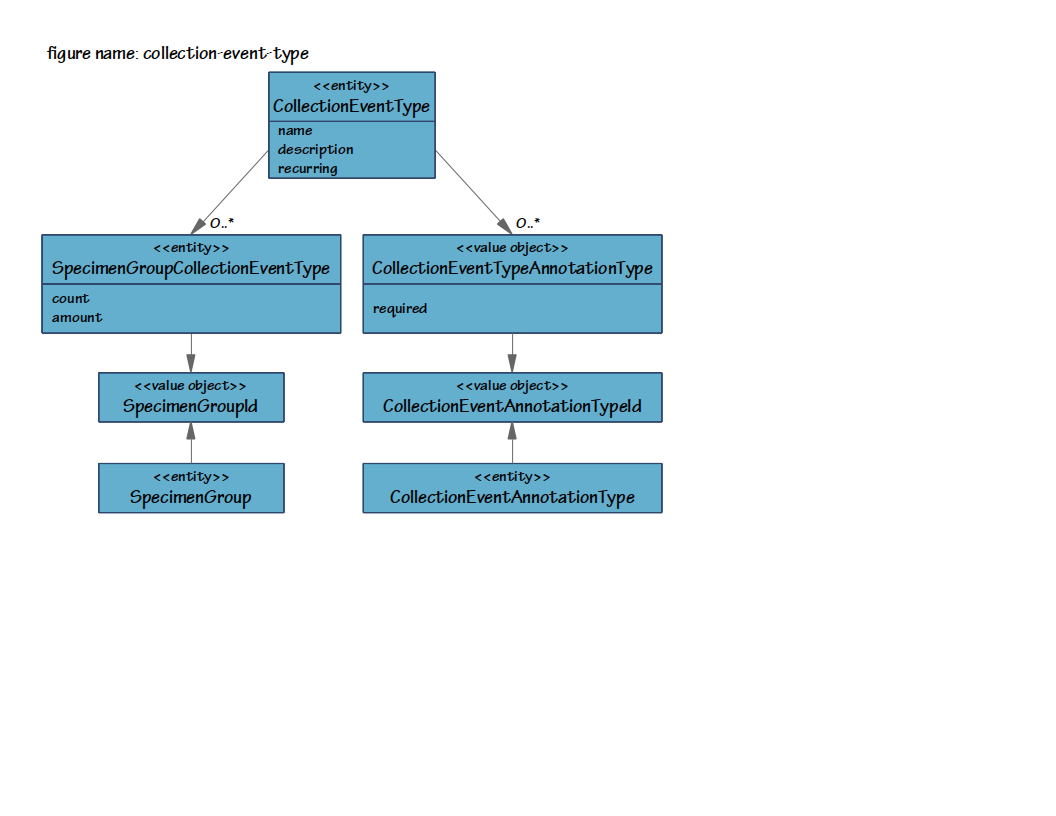
\includegraphics[trim={9mm 118mm 158mm 9mm}, clip,
    width=0.6\textwidth]{images/collection-event-type}
  \caption{Associating collection event types and specimen groups}
  \label{fig:collection-event-type}
\end{figure}

The count specifies how many specimens are to be collected. Amount is the
amount of substance that is expected in each collected specimen, or null if
there is no default amount.
\clearpage

\subsection{ProcessingType Details}
\label{sec:Processing-type}

The \texttt{\textbf{\valobjtarget{SpecimenLinkType}}} entity represents a
regularly performed processing procedure involving two \entitylink{Specimen}s:
an input, which must be in a specific \valobjlink{SpecimenGroup}, and an
output, which must be in a specific \valobjlink{SpecimenGroup}.

\begin{figure}[H]
  \centering
  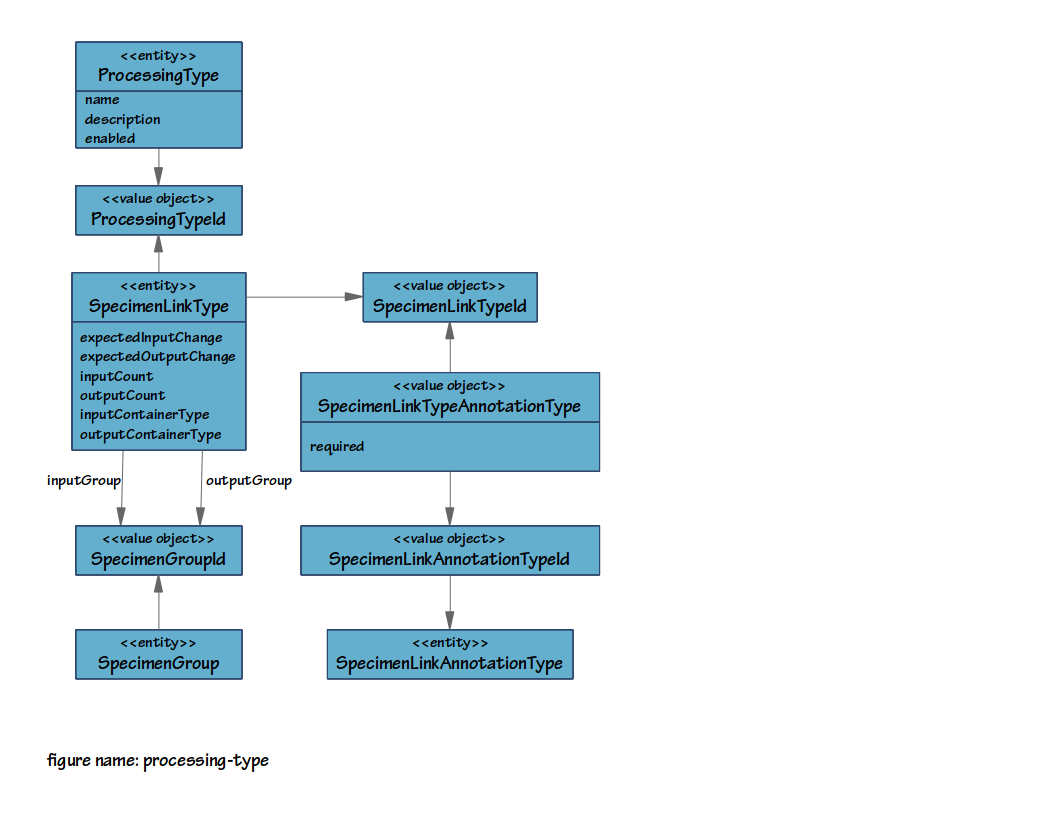
\includegraphics[trim={9mm 100mm 172mm 9mm}, clip,
    width=0.6\textwidth]{images/processing-type}
  \caption{Association processing types with specimen groups}
  \label{fig:processing-type}
\end{figure}

The expectedInputChange is the expected amount (decimal value) to be removed
from each input. The expectedOutputChange is also the expected amount to be
added to each output. The expected input and output change values can be zero.
The counts in inputCount and outputCount are the number of expected specimens
when the processing is carried out. A value of zerof for output count implies
that the count is the same as the input count. The specimen container type that
holds the input specimens is given in inputContainerType. The specimen
container type that the output specimens are stored into is given in
outputContainerType. If specifying the container types is not required for one
or both of these fields they can be assigned the \texttt{null} value.

To avoid redundancy, a specimen link type may exist only once for a given input
and output specimen group.

\section {Study Aggregate Commands}
These are the commands used to configure a study.

\begin{description}

    \item[StudyCreateCommand] \hfill \\ Used to create a study. The arguments
      are: \texttt{name (String)} and \texttt{description (String)}. The name
      used to refer to the study and is usually an acronym. The description
      describes the study and is usually the words that make up the acronym.

    \item[StudyUpdateCommand] \hfill \\ Used to create a study. The arguments
      are: \texttt{studyId (String)}, \texttt{name (String)} and
      \texttt{description (String)}. The studyId is the unique identifier for
      the study. The name contains the updated name or the current name if no
      update is required. The description contains the updated description or
      the current description if no update is required.

    \item[StudyEnableCommand] \hfill \\ Used to enable a study. Once enabled
      the study is ready to collect and process specimens from
      participants. The single argument is \texttt{studyId (String)} which is
      the unique identifier for the study.

    \item[StudyDisableCommand] \hfill \\ Used to disable a study. Once disabled
      the study can no longer collect and / or process specimens from
      participants. The single arguments is \texttt{studyId (String)} which is
      the unique identifier for the study.

    \item[CreateSpecimenGroupCommand] \hfill \\ Used to create
      a specimen group in a study. The arguments are: \texttt{studyId
	(String)}, \texttt{name (String)}, \texttt{description (String)},
      \texttt{anatomicalSourceId (String)}, \texttt{preservationId (String)},
      and \texttt{specimenTypeId (String)}. The studyId is the unique
      identifier for the study. The name describes the specimen group. The
      description provides more details for the speciment group.  The
      anatomicalSourceId is used to identify anatomical source on the
      participants whre this group belongs to.  The preservationId is used to
      record how this group is stored.  The specimenTypeId identifies the type
      of specimens contained in this group.

    \item[DeleteSpecimenGroupCommand] \hfill \\ Used to delete a specimen group
      from the study. The arguments are: \texttt{studyId (String)} and
      \texttt{specimenGroupId (String)}. The studyId is the unique identifier
      for the study. The specimenGroupId is the unique identifier for the
      specimen group.

    \item[CreateCollectionEventType] \hfill \\

    \item[DeleteCollectionEventType] \hfill \\

    \item[AddSpecimenGroupToCollectionEventType] \hfill \\

    \item[RemoveSpecimenGroupToCollectionEventType] \hfill \\

    \item[CreateProcessingType] \hfill \\

    \item[DeleteProcessingType] \hfill \\

    \item[AddSpecimenLinkType] \hfill \\

    \item[RemoveSpecimenLinkType] \hfill \\

    \item[] \hfill \\

    \item[] \hfill \\

\end{description}

